\documentclass{article}
\usepackage{tikz}
\usetikzlibrary{angles, quotes}
\usepackage{amssymb}
\usepackage{pgfplots}
\pgfplotsset{width=10cm,compat=1.9}
\usepgfplotslibrary{statistics}
\usepackage[left=2.54cm,right=2.54cm,top=2.54cm,bottom=2.54cm]{geometry}
\usepackage{tasks} %Paquete necesario para la producción de items horizontales para algunos ejercicios de tarea empleando el comando /begin{multicols}}{#}.../end{multicols} para ayudarnos a reducir las páginas
\usepackage{pdflscape} %comando que permite cambiar a orientación horizontal las hojas%
\usepackage{soul} %Paquete para permitir la compilación de acentos usando el comando {\hl{}}}\\
\sethlcolor{yellow(munsell)} %comando para definir el color para el subrayado usando el comando \hl
\usepackage[utf8]{inputenc}
\usepackage[spanish]{babel}
\usepackage{icomma}
\usepackage{ragged2e}		
\usepackage{siunitx}
\usepackage{url}
\usepackage[colorlinks=true, urlcolor=blue,  linkcolor=Cerulean, citecolor=green]{hyperref}
\usepackage{pdfpages}
\usepackage{blindtext} %Paquete que genera texto ficticio (dummy text) con el comando: \blindtext
\usepackage{cancel} %in the preamble gives you four different modes of striking through: \cancel{text to cancel} draws a diagonal line (slash) through its argument, \bcancel{text to cancel} uses the negative slope (a backslash), \xcancel{text to cancel} draws an X (actually \cancel plus \bcancel), \cancelto{〈value〉}{〈expression〉} draws a diagonal arrow through the 〈expression〉pointing to the 〈value〉 (math-mode only)
\usepackage{csquotes}
\usepackage{afterpage}
\usepackage{parskip} 
\usepackage{float}
\usepackage{enumitem}
%\usepackage{multicol}%Paquete que permite la creación aislada de columnas de texto. De esta forma se reduce la cantidad de páginas en nuestro documento
\usepackage{lipsum} %Paquete que genera texto de relleno al igual que \usepackage{blindtext}, se usa con el comando \lipsum[#-#] los #(hashtags) delimitan el número de páginas que deseamos ocupar del paquete lipsum para usarlos como relleno. 

% Definir el comando personalizado para la nota
\newcommand{\mynote}[1]{%
\begin{tikzpicture}[baseline=-0.75ex]
\node[draw, circle, fill=Apple Green!60, inner sep=2pt] (note) {\textbf{Nota:}};
\end{tikzpicture}%
\ \textit{#1}%
}

% Definición de comandos para variables con barra
\newcommand{\xbar}{\overline{x}}
\newcommand{\ybar}{\overline{y}}

\newenvironment{Figura}
{\par\medskip\noindent\minipage{\linewidth}}
{\endminipage\par\medskip}
\usepackage{caption}
\usepackage[
backend=biber,
sorting=none,
url=true
]{biblatex} %bibliografía
\addbibresource{biblio.bib}
% Establecer el espacio entre las entradas de la bibliografía
\setlength{\bibitemsep}{1\baselineskip} % Puedes ajustar el valor según tus preferencias
\usepackage{amsmath,amsthm,amssymb,amsfonts}
\usepackage{pifont} %Permite la compilación del comando \xmark: es el símbolo de la tachita
\usepackage{mathtools} %permite la compilación de símbolos para matrices
\usepackage{empheq} %Paquete que se relaciona con \usepackage[most]{tcolorbox} para la creación de cuadros/cajas de colores para delimitar los resultados matemáticos o líneas de texto usando la línea de comando: \begin{empheq}[box={\mymath[colback=orange(webcolor)!70,drop lifted shadow]}]{equation*} \end{empheq}
\usepackage[most]{tcolorbox} %Paquete que se relaciona con \usepackage{empheq} para la creación de cuadros/cajas de colores para delimitar los resultados matemáticos o líneas de texto
\renewcommand{\qedsymbol}{$\blacksquare$}
\usetikzlibrary{positioning,decorations.pathreplacing} %Paquete que permite la compilación de llaves para cuadros sinópticos (brace diagram) 
\usepackage{schemata} %The schemata package is designed just for these brace diagrams
\usepackage{booktabs}

\newcommand\AB[2]{\schema{\schemabox{#1}}{\schemabox{#2}}} %comando o paquete necesario para crear cuadros sinópticos

\newtcbox{\mymath}[1][]{%
nobeforeafter, math upper, tcbox raise base,
enhanced, colframe=blue!30!black,
colback=blue!30, boxrule=1pt,
#1} %Comando importante para encasillar los resultados matemáticos en cajas de diferentes colores, se relaciona con los paquetes \usepackage{empheq} y \usepackage[most]{tcolorbox} 

\newenvironment{sysmatrix}[1]
{\left(\begin{array}{@{}#1@{}}}
{\end{array}\right)}
\newcommand{\ro}[1]{%
\xrightarrow{\mathmakebox[\rowidth]{#1}}%
}
\newlength{\rowidth}% row operation width
\AtBeginDocument{\setlength{\rowidth}{3em}}  %Comando importante para laproducción de lineas de operaciones entre matrices, método de Gauss o Gauss Jordan se relaciona con \newenvironment{sysmatrix}

%formato para cambiar el horario a español
\usepackage[spanish]{datetime2}
\DTMsetdatestyle{spanish}

\renewcommand{\today}{\DTMdisplaydate{\the\year}{\the\month}{\the\day }{-1}}
%%%%%%%%%%%%%%%%%%%%%%%%%%%%%%%%%%%%%%%%%

\usepackage{datetime}
\newcommand{\mycurrenttime}{\xxivtime}

%%%%%%%%%%%%%%%%%%%%%%%%%%%%%%%%%%%%%%%%%%%%%%%%%%%%%%%%%%%%%%%%%%%%%%%%%%%%%%%%%%%%%%%%%%%%%%%%%%%%%%%%%%%%%%%%%%%%%%%%%%%%%%%%%%%%%%%%%%%%%%%%%


%%%%%%%%%%%%%Caja de color para el título%%%%%%%%%%%%%%%%%%%%%%%%%%%%%%%%%%%%%%%%%%%%%%%%%%%%%%

\definecolor{myframecolor}{RGB}{1, 45, 75} % Prussian Blue
\definecolor{myboxcolor}{RGB}{0, 107, 92} % Apple Green

\newtcolorbox{mybox}{
enhanced,
colback=myboxcolor!7, % Color de fondo del cuadro
colframe=myframecolor, % Color del marco del cuadro
arc=0pt,
boxrule=1pt,
borderline west={2mm}{-10mm}{myframecolor}, % Borde en el lado izquierdo
sharp corners=southwest,
width=\linewidth,
before=\par\vspace{\bigskipamount}, % Espacio antes del cuadro
after=\par\vspace{\bigskipamount} % Espacio después del cuadro
}

%%%%%%%%%%%%%%%%%%%%%%%%%%%%%%%%%%%%%%%%%%%%%%%%%%%%%%%%%Nueva caja%%%%%%%%%%%%%%%%%%%%%%%%%%%%%%%%%%%%%%%%%%%%%%%%%%%%%%%%%%%%%%%%%

\newtcolorbox{mybox2}{
enhanced,
colback=Apple Green!7, % Color de fondo del cuadro
colframe=Apple Green, % Color del marco del cuadro
arc=0pt,
boxrule=1pt,
borderline west={2mm}{-10mm}{Apple Green}, % Borde en el lado izquierdo
sharp corners=southwest,
width=\linewidth,
before=\par\vspace{\bigskipamount}, % Espacio antes del cuadro
after=\par\vspace{\bigskipamount} % Espacio después del cuadro
}


\newcommand{\euler}{e} %Comando para producir letra e de euler
\newenvironment{remark}{\par\vfill\footnotesize % Vertical white space above the remark and smaller font size
\begin{list}{}{
	\leftmargin=80pt % Indentation on the left
	\rightmargin=60pt}\item\ignorespaces % Indentation on the right
\makebox[-2.5pt]{\begin{tikzpicture}[overlay]
		\node[draw=Horizon!60,line width=2.5pt,circle,fill=Horizon!25,font=\sffamily\bfseries,inner sep=4pt,outer sep=0pt] at (-19pt,5pt){\textcolor{Horizon}{Nota}};\end{tikzpicture}} % Blue Nota in a circle
\advance\baselineskip -1pt}{\end{list}\vskip5pt} % Tighter line spacing and white space after remark
\usepackage{graphicx}

\usepackage{titling}

\input{colores.tex}

%%Producir signos de cita textual``Asignatura''

\newcommand{\xmark}{\ding{55}} %%%comando que genera la tachita

\newenvironment{MyColorPar}[1]{%
\leavevmode\color{#1}\ignorespaces%
}{%
}%

%%%%%%%%%%%%%%%%%%% Título de la tarea, Nombre de alumno

\title{ \textcolor{Sun}{\textbf{Ejercicios de repaso: \textcolor{Cinnabar}{\textbf{fonones}}}}}
\author{\emph{Tarea} $\boldsymbol{\mid}$ \textcolor{Tarawera}{\textbf{Fonones}}}
\date{\today}

%%%%%%%%%%%%%%%%%%% Datos de la Materia

\usepackage{fancyhdr}
\fancypagestyle{plain}{%  the preset of fancyhdr 
\fancyhf{} % clear all header and footer fields
\fancyfoot[R]{
\includegraphics[width=2cm]{LogoFCFMBUAP (1).png}}
\fancyfoot[L]{{\bfseries{\thedate{}}} a las {\bfseries{\mycurrenttime{}}} horas{} (GMT-6, H. Puebla de Zaragoza, Pue)}
\fancyhead[L]{\textbf{Asignatura:} Estado Sólido}
\fancyhead[R]{\theauthor}
}
\makeatletter
\def\@maketitle{%
\newpage
\null%
\begin{center}%
\let \footnote \thanks
{\LARGE \@title \par}%
\vskip 1em%
%{\large \@date}%
\end{center}%
}
\makeatother

\usepackage{lipsum}  
\usepackage{cmbright}


%%%%%%%%%%%%%%%%%%%%%%%%%%%%%%%%%%%%%%%%%%%%%%%%%%%%%%%%%%%%%%%%%%%%%%%%%%%%%%%%%%%%%%%%%%%%%%%%%%%%%%%%%%%%%%%%%%%%%%%%%%%%%%%%%%%%%%%%%%%%%%%%%%%%%%%%%%%%%%%%%%%%%%%%%%%%%%%%%%%%%%%%%%%%%%%%%%%%%%

% Por si el color se llama "Apple Green" con espacio en colores.tex:
\colorlet{AppleGreen}{Apple Green}

% Caja AppleGreen con tono ajustable
\newenvironment{AGbox}[1][7]% 7 = tono por defecto (más grande => más claro)
{%
  \begin{tcolorbox}[
    enhanced, breakable,
    colframe=AppleGreen,
    colback=AppleGreen!#1,
    boxrule=1pt,
    borderline west={2mm}{-10mm}{AppleGreen},
    sharp corners=southwest,
    left=14pt,right=14pt,top=10pt,bottom=10pt,
     boxsep=6pt,
  ]%
}{%
  \end{tcolorbox}%
}


\begin{document}



\maketitle

%%%%%%%%%%%%%%%%%%% Datos del profesor, campus, aula e integrantes

\begin{mybox2}
\noindent
\begin{tabular}{@{}p{3.7cm}p{10.4cm}@{}}
\textbf{Profesor} & Dra. Ana Lilia González Ronquillo \\[3pt]
\textbf{Campus / Facultad} & \textcolor{prussianblue}{\textbf{C.U. BUAP}} / \textcolor{trueblue}{\textbf{FCFM}} \\[3pt]
\textbf{Edificio / Salón} & \textcolor{prussianblue}{\textbf{FM9}} / \textcolor{trueblue}{\textbf{301}} \\[6pt]
\textbf{Alumno} & Julio Alfredo Ballinas García
\end{tabular}
\end{mybox2}
\vspace{1cm}


\vspace{0.5cm}
\begin{center}
\begin{tikzpicture}
	% Dibuja círculos rellenos en diferentes colores
	\fill[bittersweet] (0,0) circle (0.17cm);
	\fill[Apple Green] (0.6,0) circle (0.17cm);
	\fill[trueblue] (1.2,0) circle (0.17cm);
	\fill[Aguamarina] (1.8,0) circle (0.17cm);
	\fill[Sun] (2.4,0) circle (0.17cm);
	\fill[orange(colorwheel)] (3.0,0) circle (0.17cm);
	\fill[Pesto] (3.6,0) circle (0.17cm);
	\fill[blue-violet] (4.2,0) circle (0.17cm);
	\fill[ticklemepink] (4.8,0) circle (0.17cm);
	\fill[Gallery] (5.4,0) circle (0.17cm);
	\fill[Mantle] (6.0,0) circle (0.17cm);
	\fill[Nevada] (6.6,0) circle (0.17cm);
	\fill[onyx] (7.2,0) circle (0.17cm);
	% Agrega más círculos o modifica los colores según sea necesario
\end{tikzpicture}
\end{center}  \vspace{0.5cm}

\setlength{\columnsep}{2cm}
%\begin{multicols}{2}
\section*{\textcolor{Tarawera}{\textbf{Lista de problemas y soluciones}}}
\addcontentsline{toc}{section}{\textcolor{Tarawera}{\textbf{Problemas:  Fonones}}}

%=============================
% PR. 3.1 — Modos normales con constantes alternadas
%=============================
\begin{AGbox}[8]
\begin{enumerate}[label={{\textcolor{trueblue}{\textbf{Pr.} \arabic*.1}}}, start=1]
  \item Considere los modos normales de una cadena lineal en la cual las constantes del resorte son alternadamente $c$ y $10c$. Sea la masa de los átomos $m$ y la distancia entre primeros vecinos $a/2$. Encontrar la relación de dispersión $\omega(k)$ para $k = 0$ y $k = \pi / a$.
\end{enumerate}
\end{AGbox}

\textcolor{Cinnabar}{\textbf{Solución:}}

\noindent\textbf{Modelo y notación}\; La cadena es monoatómica con masas iguales $m$ separadas por $a/2$, pero los enlaces alternan su rigidez: entre $A_n$ y $B_n$ la constante es $K_1=c$, y entre $B_n$ y $A_{n+1}$ la constante es $K_2=10c$. La periodicidad de la \emph{celda} es $a$ y contiene dos átomos: $A_n$ y $B_n$

\noindent\textbf{Ecuaciones de movimiento}\;
Sean $u_n(t)$ y $v_n(t)$ los desplazamientos longitudinales de $A_n$ y $B_n$. Las fuerzas sobre cada masa dependen de las diferencias de desplazamiento con sus vecinos conectados por resortes:
\begin{equation}
m\,\ddot u_n \;=\; -K_1(u_n - v_n) - K_2(u_n - v_{n-1}) \;=\; -(K_1+K_2)u_n + K_1 v_n + K_2 v_{n-1}
\label{eq:pr31_eom_u}
\end{equation}
\begin{equation}
m\,\ddot v_n \;=\; -K_1(v_n - u_n) - K_2(v_n - u_{n+1}) \;=\; -(K_1+K_2)v_n + K_1 u_n + K_2 u_{n+1}
\label{eq:pr31_eom_v}
\end{equation}

\noindent\textbf{Ansatz de ondas planas}\;
Buscamos modos normales del tipo
\begin{equation}
u_n(t)=u\,e^{i(kna-\omega t)}, \qquad v_n(t)=v\,e^{i(kna-\omega t)}
\label{eq:pr31_ansatz}
\end{equation}
de donde $v_{n-1}=v\,e^{-ika}\,e^{i(kna-\omega t)}$ y $u_{n+1}=u\,e^{ika}\,e^{i(kna-\omega t)}$. Sustituyendo \eqref{eq:pr31_ansatz} en \eqref{eq:pr31_eom_u}–\eqref{eq:pr31_eom_v} y factorizando $e^{i(kna-\omega t)}$ llegamos al sistema lineal
\begin{equation}
\big(m\omega^2 - (K_1+K_2)\big)\,u \;+\; \big(K_1 + K_2 e^{-ika}\big)\,v \;=\; 0
\label{eq:pr31_mat1}
\end{equation}
\begin{equation}
\big(K_1 + K_2 e^{ika}\big)\,u \;+\; \big(m\omega^2 - (K_1+K_2)\big)\,v \;=\; 0
\label{eq:pr31_mat2}
\end{equation}
que se escribe matricialmente como $M(k,\omega)\,(u,v)^{\top}=0$ con
\[
M(k,\omega)=
\begin{pmatrix}
m\omega^2-(K_1+K_2) & K_1 + K_2 e^{-ika}\\
K_1 + K_2 e^{ika}   & m\omega^2-(K_1+K_2)
\end{pmatrix}
\]

\noindent\textbf{Condición de dispersión}\;
Para soluciones no triviales se requiere $\det M=0$:
\begin{equation}
\big(m\omega^2-(K_1+K_2)\big)^2 - \big(K_1 + K_2 e^{-ika}\big)\big(K_1 + K_2 e^{ika}\big)=0
\label{eq:pr31_det0}
\end{equation}
Observa que
\begin{equation}
\big(K_1 + K_2 e^{-ika}\big)\big(K_1 + K_2 e^{ika}\big)=K_1^2 + K_2^2 + 2K_1K_2\cos(ka)
\label{eq:pr31_prod}
\end{equation}
Usando \eqref{eq:pr31_prod} en \eqref{eq:pr31_det0} se obtiene inmediatamente la relación de dispersión de las dos ramas
\begin{equation}
\boxed{\;\omega^2(k)=\frac{K_1+K_2}{m}\;\pm\;\frac{1}{m}\sqrt{\,K_1^2+K_2^2+2K_1K_2\cos(ka)\,}\;}
\label{eq:pr31_disp_general}
\end{equation}

\noindent\textbf{Evaluación en $k=0$}\; Aquí $\cos(0)=1$ y $\sqrt{K_1^2+K_2^2+2K_1K_2} = K_1+K_2$, por lo que
\begin{equation}
\omega^2(0)=\frac{K_1+K_2}{m}\;\pm\;\frac{K_1+K_2}{m}
\;\;\Rightarrow\;\;
\boxed{\;\omega(0)=0\;}\quad\text{(rama acústica)},\qquad
\boxed{\;\omega^2(0)=\frac{2(K_1+K_2)}{m}\;}
\label{eq:pr31_k0}
\end{equation}

\noindent\textbf{Evaluación en $k=\pi/a$}\; Aquí $\cos(\pi)=-1$ y
$\sqrt{K_1^2+K_2^2-2K_1K_2}=\lvert K_1-K_2\rvert$, de modo que
\begin{equation}
\omega^2\!\left(\frac{\pi}{a}\right)=\frac{K_1+K_2}{m}\;\pm\;\frac{|K_1-K_2|}{m}
\;=\;\Big\{\;\frac{2K_{\min}}{m}\;,\;\frac{2K_{\max}}{m}\;\Big\}
\label{eq:pr31_kpia}
\end{equation}

\noindent\textbf{Sustituyendo $K_1=c$ y $K_2=10c$}\;
\begin{equation}
\boxed{\;\omega(0)=0\;,\qquad \omega(0)=\sqrt{\frac{2(11c)}{m}}=\sqrt{\frac{22c}{m}}\;}
\label{eq:pr31_final_0}
\end{equation}
\begin{equation}
\boxed{\;\omega^2\!\left(\frac{\pi}{a}\right)=\frac{2c}{m}\;,\;\frac{20c}{m}
\quad\Rightarrow\quad
\omega\!\left(\frac{\pi}{a}\right)=\sqrt{\frac{2c}{m}}\;,\;\sqrt{\frac{20c}{m}}\;}
\label{eq:pr31_final_pia}
\end{equation}

\noindent\textbf{Comentario físico}\; En $k=0$ las masas se mueven en fase: el modo es acústico y la frecuencia se anula. En $k=\pi/a$ las masas vecinas vibran en antifase; los dos valores corresponden a “endurecer” la celda con el enlace más rígido o el más débil, de ahí que aparezcan $2K_{\max}/m$ y $2K_{\min}/m$




\vspace{0.5cm}

%=============================
% PR. 3.2 — Propagación de ondas longitudinales monoatómicas (vecinos hasta j-ésimos)
%=============================
\begin{AGbox}[8]
\begin{enumerate}[label={{\textcolor{trueblue}{\textbf{Pr.} \arabic*.2}}}, start=1]
  \item Considere la propagación de ondas longitudinales a lo largo de una cadena lineal monoatómica. La masa de cada átomo es $m$, el espaciamiento atómico en equilibrio es $a$, y la constante del resorte con respecto al vecino $j$-ésimo es $\mu_j$. Mostrar que cuando se considera interacción con vecinos más allá de los primeros vecinos, la relación de dispersión es:
  \begin{equation}
    \omega^2 = \frac{2}{m} \sum_{j=1}^{\infty} \mu_j \, [1 - \cos(jka)]
    \label{eq:dispersion_vecinos}
  \end{equation}
\end{enumerate}
\end{AGbox}

\textcolor{Cinnabar}{\textbf{Solución:}}

\noindent\textbf{Modelo físico y fuerzas elásticas}\;
Cada partícula $n$ (de masa $m$) está unida con resortes a sus vecinos $\pm j$ ($j=1,2,\dots$). Si $u_n(t)$ es el desplazamiento longitudinal de la partícula $n$, la contribución del par de resortes que conectan $n$ con $n\pm j$ es proporcional a la \emph{elongación relativa} $u_{n\pm j}-u_n$. Por simetría izquierda–derecha, las fuerzas se agrupan como diferencias centradas:
\begin{equation}
  m\,\ddot u_n
  \;=\;
  \sum_{j=1}^{\infty} \mu_j \,\big[\, (u_{n+j}-u_n) + (u_{n-j}-u_n) \,\big]
  \;=\;
  \sum_{j=1}^{\infty} \mu_j \,\big(u_{n+j}+u_{n-j}-2u_n\big)
  \label{eq:pr32_eom}
\end{equation}

\noindent\textbf{Modos normales (ondas planas)}\;
Buscamos soluciones del tipo
\begin{equation}
  u_n(t) = u\,e^{\,i(kna-\omega t)}
  \label{eq:pr32_ansatz}
\end{equation}
de donde
\(
u_{n\pm j} = u\,e^{\,i(k(n\pm j)a-\omega t)} = u\,e^{\,\pm i jka}\,e^{\,i(kna-\omega t)}
\).
Sustituyendo \eqref{eq:pr32_ansatz} en \eqref{eq:pr32_eom} y factorizando el factor común $e^{\,i(kna-\omega t)}$:
\begin{equation}
  -\,m\,\omega^2\,u
  \;=\;
  \sum_{j=1}^{\infty} \mu_j \,\big(\,e^{\,i jka}+e^{\,-i jka}-2\,\big)\,u
  \label{eq:pr32_pretrigo}
\end{equation}

\noindent\textbf{Uso de identidades trigonométricas}\;
Con Euler, $e^{ix}+e^{-ix}=2\cos x$, por lo que
\begin{equation}
  e^{\,i jka}+e^{\,-i jka}-2
  \;=\;
  2\cos(jka)-2
  \;=\;
  -\,2\,[\,1-\cos(jka)\,]
  \label{eq:pr32_trigo}
\end{equation}
Sustituyendo \eqref{eq:pr32_trigo} en \eqref{eq:pr32_pretrigo} y dividiendo por $u\neq 0$:
\begin{equation}
  m\,\omega^2
  \;=\;
  2\sum_{j=1}^{\infty}\mu_j\,[\,1-\cos(jka)\,]
  \quad\Rightarrow\quad
  \boxed{\;
    \omega^2(k) \;=\; \frac{2}{m} \sum_{j=1}^{\infty} \mu_j \,[\,1 - \cos(jka)\,]
  \;}
  \label{eq:pr32_disp_final}
\end{equation}

\noindent\textbf{Comprobaciones y casos límite}\;
(i) Si sólo hay primeros vecinos ($\mu_1=\beta$, $\mu_{j>1}=0$) se recupera la expresión estándar
\(
\omega^2=\frac{2\beta}{m}[\,1-\cos(ka)\,]
\)
\; (consistente con el caso monoatómico de primer vecino)\;
(ii) Para $ka\ll 1$, usando $\cos(jka)\simeq 1-(jka)^2/2$, se obtiene una ley lineal $\omega\simeq v\,k$ con
\(
v=a\,\sqrt{\tfrac{1}{m}\sum_{j} j^2\mu_j}
\),
lo que muestra cómo los acoplos de mayor alcance aumentan la pendiente acústica en el régimen de ondas largas


%=============================
% PR. 3.3 — Vibraciones en una red cuadrada plana (2D)
%=============================
\begin{AGbox}[8]
\begin{enumerate}[label={{\textcolor{trueblue}{\textbf{Pr.} \arabic*.3}}}, start=1]
  \item Considere átomos idénticos que vibran en una \textbf{red cuadrada plana} de paso $a$ y masa atómica $m$. La constante del resorte (interacción con primeros vecinos) es $\beta$ 
  \begin{figure}[H]
    \centering
    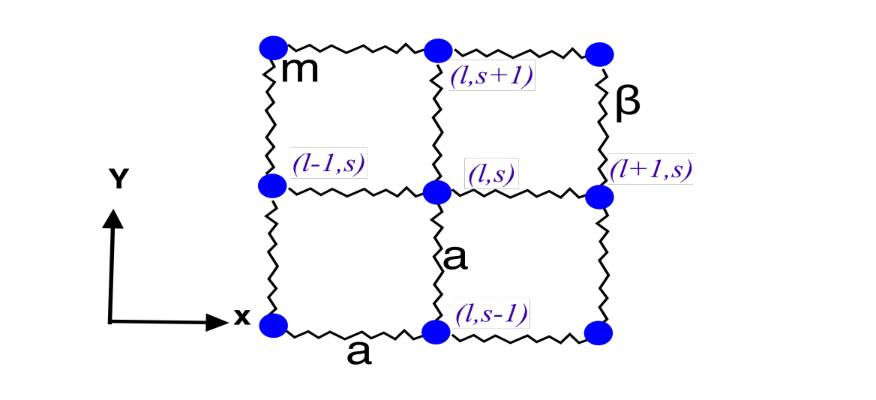
\includegraphics[width=0.8\textwidth]{red_cuadrada_plana.png}% <-- sustituye por tu nombre de archivo
    \caption{Esquema de una red cuadrada plana con vecinos en $\pm \hat x$ y $\pm \hat y$}
    \label{fig:red_cuadrada_2D}
  \end{figure}

  \begin{enumerate}[label=\textbf{(\alph*)}]
  \item \textbf{Ecuación de movimiento}

  Numeremos los sitios por dos enteros $(l,s)$ que identifican columna y fila. Denotemos por $u_{l,s}(t)$ el desplazamiento del átomo en $(l,s)$ en la dirección de la vibración considerada. Con interacción de \emph{primeros vecinos} y constante de resorte $\beta$, la fuerza resultante es la suma de cuatro contribuciones tipo Hooke, cada una proporcional a la \emph{elongación relativa} con respecto a un vecino
  \[
    F_{l,s}
    \;=\;
    \beta\big[(u_{l+1,s}-u_{l,s})+(u_{l-1,s}-u_{l,s})+(u_{l,s+1}-u_{l,s})+(u_{l,s-1}-u_{l,s})\big]
  \]
  Agrupando términos semejantes se reconoce la suma de dos “Laplacianos” 1D centrados, uno en $x$ y otro en $y$
  \begin{equation}
    m\,\frac{d^{2}u_{l,s}}{dt^{2}}
    \;=\;
    \beta\Big[(u_{l+1,s}+u_{l-1,s}-2u_{l,s})+(u_{l,s+1}+u_{l,s-1}-2u_{l,s})\Big]
    \label{eq:mov_red_cuadrada}
  \end{equation}

  \item \textbf{Relación de dispersión a partir de una onda plana}

  Buscamos un modo normal como onda plana en 2D
  \begin{equation}
    u_{l,s}(t)=u_0\,
    \exp\!\big[i(lk_x a + s k_y a - \omega t)\big]
    \label{eq:onda_plana_2D}
  \end{equation}
  De \eqref{eq:onda_plana_2D} se sigue que
  \[
    u_{l\pm1,s}=u_{l,s}\,e^{\pm i k_x a}
    \qquad\text{y}\qquad
    u_{l,s\pm1}=u_{l,s}\,e^{\pm i k_y a}
  \]
  Sustituyendo en \eqref{eq:mov_red_cuadrada} y dividiendo por el factor común $u_{l,s}$ se obtiene
  \[
    -\,m\omega^2
    \;=\;
    \beta\big[\,(e^{ik_xa}+e^{-ik_xa}-2)+(e^{ik_ya}+e^{-ik_ya}-2)\,\big]
  \]
  Usando $e^{ix}+e^{-ix}=2\cos x$, resulta
  \begin{equation}
    \boxed{\,\omega^{2}(k_x,k_y)
    \;=\;
    \frac{2\beta}{M}\,\Big[\,2-\cos(k_x a)-\cos(k_y a)\,\Big]\,}
    \label{eq:dispersion_2D}
  \end{equation}
  con $M=m$ la masa de cada átomo. Esta es la análoga 2D del resultado 1D monoatómico $\,\omega^2=\tfrac{2\beta}{m}\,[1-\cos(ka)]\,$ que ya conoces de la cadena lineal

  \item \textbf{Límite de ondas largas: $\;ka\ll 1$}

  Para vectores de onda pequeños se usa la expansión $\cos\alpha\simeq 1-\alpha^2/2$. Aplicándola a \eqref{eq:dispersion_2D}
  \[
    2-\cos(k_x a)-\cos(k_y a)
    \;\simeq\;
    2-\Big(1-\tfrac{(k_x a)^2}{2}\Big)-\Big(1-\tfrac{(k_y a)^2}{2}\Big)
    \;=\;\frac{a^2}{2}(k_x^2+k_y^2)
  \]
  Por tanto
  \begin{equation}
    \omega^2 \;\simeq\; \frac{2\beta}{M}\cdot\frac{a^2}{2}\,(k_x^2+k_y^2)
    \;=\; \frac{\beta a^2}{M}\,(k_x^2+k_y^2)
    \label{eq:dispersion_2D_peqk}
  \end{equation}
  Definiendo $k=\sqrt{k_x^2+k_y^2}$, se concluye
  \begin{equation}
    \boxed{\,\omega \;\simeq\; v\,k\,,\qquad v \;=\; a\,\sqrt{\frac{\beta}{M}}\,}
    \label{eq:lineal_baja_k}
  \end{equation}
  es decir, \emph{dispersión lineal} en el régimen acústico de ondas largas. La velocidad $v$ coincide con la pendiente de $\omega(k)$ en el entorno de $\Gamma$ y es la velocidad de propagación de la perturbación elástica en esta red 2D
  \end{enumerate}
\end{enumerate}
\end{AGbox}



%=============================
% PR. 3.4 — Einstein 2D: C_v a volumen constante
%=============================
\begin{AGbox}[8]
\begin{enumerate}[label={{\textcolor{trueblue}{\textbf{Pr.} \arabic*.4}}}, start=1]
  \item Calcular el \textbf{calor específico a volumen constante} para un \textbf{material bidimensional}. Use el \textbf{modelo de Einstein} y haga un análisis a \textbf{bajas} y \textbf{altas} temperaturas.
\end{enumerate}
\end{AGbox}

\textcolor{Cinnabar}{\textbf{Solución:}}

\noindent\textbf{Idea del modelo de Einstein en 2D}\;
Un sólido 2D con $N$ átomos tiene \textit{dos} grados vibracionales por átomo en el plano, por lo que el número total de osciladores independientes es $2N$. El modelo de Einstein asume que \emph{todas} las oscilaciones tienen la misma frecuencia $\omega_E$. El espectro está, pues, \textit{degenerado} en una sola frecuencia

\noindent\textbf{Energía media por oscilador}\;
Ignorando la energía de punto cero (no contribuye a $C_V$), la energía térmica media de un oscilador cuántico armónico a frecuencia fija $\omega_E$ es
\begin{equation}
  \langle \varepsilon \rangle \;=\; \frac{\hbar \omega_E}{e^{\hbar\omega_E/k_B T}-1}
  \label{eq:e_media_osc}
\end{equation}

\noindent\textbf{Energía interna total en 2D}\;
Multiplicando por el número total de osciladores $2N$ se obtiene
\begin{equation}
  U(T) \;=\; 2N \,\frac{\hbar \omega_E}{e^{\hbar\omega_E/k_B T}-1}
  \label{eq:U_Einstein2D}
\end{equation}
Es útil definir la \emph{temperatura de Einstein} $\Theta_E=\hbar\omega_E/k_B$ y la variable adimensional $x=\Theta_E/T$, con lo cual
\begin{equation}
  U(T) \;=\; 2N\,k_B T \,\frac{x}{e^{x}-1}
  \label{eq:U_Einstein2D_x}
\end{equation}

\noindent\textbf{Calor específico a volumen constante}\;
Derivando \eqref{eq:U_Einstein2D} respecto a $T$ (a volumen constante) se obtiene
\begin{equation}
  C_V \;=\; \left(\frac{\partial U}{\partial T}\right)_{V}
  \;=\;
  2N k_B \left(\frac{\hbar\omega_E}{k_B T}\right)^{\!2}
  \frac{e^{\hbar\omega_E/k_B T}}{\big(e^{\hbar\omega_E/k_B T}-1\big)^{\!2}}
  \;=\;
  2N k_B \,\frac{x^{2} e^{x}}{(e^{x}-1)^{2}}
  \label{eq:Cv_Einstein2D}
\end{equation}

\noindent\textbf{Límite de \underline{altas temperaturas}} $\,(T\gg \Theta_E)$\;
Cuando $x=\Theta_E/T \ll 1$, se usa $e^{x}\approx 1+x+\tfrac{x^2}{2}+\cdots$ y se verifica que
\begin{equation}
  \frac{x^{2} e^{x}}{(e^{x}-1)^{2}} \;\longrightarrow\; 1
  \qquad\Rightarrow\qquad
  \boxed{\,C_V \;\xrightarrow[T\gg \Theta_E]{}\; 2N\,k_B\,}
  \label{eq:Cv_altaT}
\end{equation}
Este es el análogo 2D de la ley de Dulong–Petit: dos grados vibracionales por átomo aportan $k_B$ cada uno

\noindent\textbf{Límite de \underline{bajas temperaturas}} $\,(T\ll \Theta_E)$\;
Para $x\gg 1$, $e^{x}\gg 1$ y se tiene
\begin{equation}
  \frac{x^{2} e^{x}}{(e^{x}-1)^{2}}
  \;\simeq\;
  x^{2}e^{-x}
  \qquad\Rightarrow\qquad
  \boxed{\,C_V \;\xrightarrow[T\ll \Theta_E]{}\; 2N\,k_B\,x^{2}e^{-x}
  \;=\; 2N\,k_B\left(\frac{\Theta_E}{T}\right)^{\!2} e^{-\Theta_E/T}\,}
  \label{eq:Cv_bajaT}
\end{equation}
Es decir, el calor específico cae \emph{exponencialmente} a bajas temperaturas en el modelo de Einstein (al no haber modos acústicos dispersivos que alimenten una ley de potencia)

\noindent\textbf{Resumen operativo}\;
\begin{equation}
  U(T) \;=\; 2N\,\frac{\hbar\omega_E}{e^{\hbar\omega_E/k_B T}-1}
  \qquad
  C_V(T) \;=\; 2N k_B \,\frac{x^{2} e^{x}}{(e^{x}-1)^{2}}
  \qquad
  x=\frac{\Theta_E}{T}
  \label{eq:Einstein2D_resumen}
\end{equation}
\begin{equation}
  C_V \;\to\; 2N k_B \quad (T\gg \Theta_E)
  \qquad\qquad
  C_V \;\sim\; 2N k_B \left(\frac{\Theta_E}{T}\right)^2 e^{-\Theta_E/T} \quad (T\ll \Theta_E)
  \label{eq:Einstein2D_resumen_lim}
\end{equation}


\vspace{0.5cm}

%=============================
% PR. 3.5 — Debye 2D: densidad de modos, $\omega_D$, $U(T)$ y $C_v$
%=============================
\begin{AGbox}[8]
\begin{enumerate}[label={{\textcolor{trueblue}{\textbf{Pr.} \arabic*.5}}}, start=1]
  \item Use el \textbf{modelo de Debye} para determinar el \textbf{calor específico a volumen constante} de un \textbf{material bidimensional}. Suponga que se satisface la relación de dispersión $\omega(k)=v k$ y proceda así:
  \begin{enumerate}[label=\textbf{(\alph*)}]
    \item Hallar una expresión para la \textbf{densidad de modos} $g(\omega)$.
    \item Encontrar una expresión para la \textbf{frecuencia de Debye}, $\omega_D$.
    \item Determinar la \textbf{energía interna} $U(T)$.
    \item Hacer un \textbf{análisis de $U$ a altas temperaturas} y determinar el \textbf{calor específico} correspondiente.
    \item Hacer un \textbf{análisis de $U$ a bajas temperaturas} y determinar el \textbf{calor específico} correspondiente.
  \end{enumerate}
\end{enumerate}
\end{AGbox}

\textcolor{Cinnabar}{\textbf{Solución:}}

\noindent\textbf{Planteamiento general}\;
En 2D, cada átomo aporta dos polarizaciones acústicas (dos direcciones de vibración). Por tanto, un cristal bidimensional con $N$ átomos posee \textbf{2N modos acústicos}. En el \textbf{modelo de Debye}, se aproxima la dispersión por una ley lineal:
\[
\omega(k)=v\,k
\]
lo cual es válido en la región de \textit{ondas largas}, es decir, cerca del punto $\Gamma$.

%-------------------------------------------------------------
\subsubsection*{\textbf{(a) Densidad de modos $g(\omega)$}}
En 2D, el espacio recíproco se llena uniformemente. El número de estados con número de onda menor que $k$ es proporcional al área del disco de radio $k$:
\[
N(k) = (\text{número de estados por unidad de área}) \times \text{Área del disco}
= \frac{A}{(2\pi)^2}\,\pi k^2
\]
donde $A$ es el área del cristal. Como hay \textbf{dos polarizaciones acústicas}, multiplicamos por 2:
\[
N_{\text{acústico}}(k) = \frac{2A}{4\pi}\,k^2 = \frac{A}{2\pi}\,k^2
\]
Derivando respecto a $k$, se obtiene la densidad de estados en $k$:
\[
g(k)=\frac{dN}{dk}=\frac{A}{\pi}\,k
\]
Con la relación de dispersión $\omega = vk$:
\[
k=\frac{\omega}{v}, \qquad \frac{dk}{d\omega}=\frac{1}{v}
\]
Por tanto, la densidad de modos en frecuencia es
\begin{equation}
\boxed{\,g(\omega)=\frac{A}{\pi v^2}\,\omega\,}
\label{eq:debye2D_gw}
\end{equation}

%-------------------------------------------------------------
\subsubsection*{\textbf{(b) Frecuencia de Debye $\omega_D$}}
La frecuencia de Debye se define exigiendo que el número total de modos accesibles sea exactamente $2N$:
\[
\int_{0}^{\omega_D} g(\omega)\,d\omega = 2N
\]
Usando \eqref{eq:debye2D_gw}:
\[
\int_{0}^{\omega_D} \frac{A}{\pi v^2}\,\omega\,d\omega
= \frac{A}{\pi v^2}\,\frac{\omega_D^2}{2}
= 2N
\]
Despejando:
\begin{equation}
\boxed{\,\omega_D = v\,\sqrt{\frac{4\pi N}{A}}\,}
\label{eq:debye2D_wD}
\end{equation}

%-------------------------------------------------------------
\subsubsection*{\textbf{(c) Energía interna $U(T)$}}
Cada modo de frecuencia $\omega$ contribuye con energía promedio
\[
\langle \varepsilon(\omega) \rangle = \frac{\hbar\omega}{e^{\hbar\omega/k_BT}-1}
\]
Por tanto:
\[
U(T)=\int_{0}^{\omega_D} \frac{\hbar\omega\,g(\omega)}{e^{\hbar\omega/k_BT}-1}\,d\omega
\]
Sustituyendo $g(\omega)$:
\[
U(T)=\frac{A}{\pi v^2}\int_{0}^{\omega_D}\frac{\hbar\omega^2}{e^{\hbar\omega/k_BT}-1}\,d\omega
\]
Sea $x=\hbar\omega/k_BT$, entonces $d\omega=\frac{k_BT}{\hbar}dx$ y $\omega_D \rightarrow x_D=\Theta_D/T$, con $\Theta_D=\hbar\omega_D/k_B$:
\begin{equation}
\boxed{\,U(T)=\frac{A}{\pi v^2}\frac{(k_BT)^3}{\hbar^2}\int_{0}^{\Theta_D/T}\frac{x^2}{e^{x}-1}\,dx\,}
\label{eq:debye2D_U}
\end{equation}

%-------------------------------------------------------------
\subsubsection*{\textbf{(d) Altas temperaturas $T\gg \Theta_D$}}
En este caso $\Theta_D/T \ll 1$, y la integral se aproxima a su límite clásico:
\[
\int_{0}^{\Theta_D/T}\frac{x^2}{e^{x}-1}dx \;\approx\; \frac{(\Theta_D/T)^3}{3}
\]
lo que conduce a $U \approx 2Nk_BT$ y por tanto:
\begin{equation}
\boxed{\,C_V = \left(\frac{\partial U}{\partial T}\right)_V \xrightarrow[T\gg\Theta_D]{} 2N k_B\,}
\label{eq:debye2D_Cv_altaT}
\end{equation}
Este es el análogo bidimensional de la ley de Dulong–Petit.

%-------------------------------------------------------------
\subsubsection*{\textbf{(e) Bajas temperaturas $T\ll \Theta_D$}}
Para $\Theta_D/T \gg 1$:
\[
\int_{0}^{\infty}\frac{x^2}{e^{x}-1}dx = 2\zeta(3)
\]
entonces \eqref{eq:debye2D_U} da
\[
U(T)\;\propto\;T^3
\]
y al derivar:
\begin{equation}
\boxed{\,C_V \;\propto\; T^2 \qquad (T\ll \Theta_D)\,}
\label{eq:debye2D_Cv_bajaT}
\end{equation}
lo que muestra que en 2D el calor específico acústico sigue una \emph{ley cuadrática en temperatura} a bajas temperaturas.


%=============================
% PR. 3.6 — Calor específico con relación de dispersión cuadrática
%=============================
\begin{AGbox}[8]
\begin{enumerate}[label={{\textcolor{trueblue}{\textbf{Pr.} \arabic*.6}}}, start=1]
  \item Suponga que en un \textbf{sólido tridimensional} hay \textbf{ondas cuantizadas} que siguen la relación de dispersión $\omega = A k^{2}$, donde $A$ es una constante con unidades apropiadas.  
  Cuando dichas ondas son excitadas por efectos térmicos, se observa cierta cantidad de \textbf{calor específico}.  
  \begin{enumerate}[label=\textbf{(\alph*)}]
    \item Encuentre una expresión para la \textbf{densidad de modos} $g(\omega)$ considerando la relación de dispersión mencionada.  
    \item Usando
    \begin{equation}
      U = \int_{0}^{\omega_D} 
      \frac{ \hbar \omega\, g(\omega) }
      { e^{\hbar \omega / k_B T} - 1 }
      \, d\omega
      \label{eq:energia_dispersión_cuadrática}
    \end{equation}
    encuentre una expresión para la \textbf{energía interna} del sistema
    \item Derive el resultado del inciso (b) para mostrar que el \textbf{calor específico a volumen constante} es proporcional a $T^{3/2}$ a bajas temperaturas
  \end{enumerate}
\end{enumerate}
\end{AGbox}

\textcolor{Cinnabar}{\textbf{Solución:}}

\noindent\textbf{Planteamiento y conteo de estados}\;
Supondremos un medio 3D isotrópico de volumen $V$ y, salvo que se indique lo contrario, una sola rama de excitación\footnote{Si hubiese $g$ polarizaciones independientes, basta multiplicar por $g$ todas las expresiones finales}. Para periodicidad de Born–von Kármán, el número de estados con número de onda menor que $k$ es
\begin{equation}
  N(k) \;=\; \frac{V}{(2\pi)^3}\,\frac{4\pi}{3}\,k^3
  \label{eq:pr36_Nk}
\end{equation}
La densidad de estados en $k$ es
\begin{equation}
  g(k)\;=\;\frac{dN}{dk}\;=\;\frac{V}{2\pi^2}\,k^2
  \label{eq:pr36_gk}
\end{equation}

\noindent\textbf{(a) Densidad de modos $g(\omega)$ para $\omega=A k^2$}\;
De la dispersión $\,\omega=A k^2\,$ se tiene $\,k=\sqrt{\omega/A}\,$ y $\,\frac{dk}{d\omega}=\frac{1}{2\sqrt{A\omega}}$. Entonces
\begin{equation}
  g(\omega)\;=\;g(k)\,\frac{dk}{d\omega}
  \;=\;
  \frac{V}{2\pi^2}\,k^2 \cdot \frac{1}{2\sqrt{A\omega}}
  \;=\;
  \boxed{\,g(\omega)\;=\;\frac{V}{4\pi^2}\,\frac{\sqrt{\omega}}{A^{3/2}}\,}
  \label{eq:pr36_gomega}
\end{equation}
Si existen $g$ polarizaciones, reemplace $V\to g\,V$ en \eqref{eq:pr36_gomega}

\noindent\textbf{(b) Energía interna}\;
Cada modo de frecuencia $\omega$ aporta energía promedio
\begin{equation}
  \langle \varepsilon(\omega) \rangle \;=\; \frac{\hbar\omega}{e^{\hbar\omega/k_BT}-1}
  \label{eq:pr36_eps}
\end{equation}
De \eqref{eq:energia_dispersión_cuadrática} con \eqref{eq:pr36_gomega}
\begin{equation}
  U(T) \;=\; \frac{V}{4\pi^2 A^{3/2}} \int_0^{\omega_D} 
  \frac{\hbar\,\omega^{3/2}}{e^{\hbar\omega/k_BT}-1}\,d\omega
  \label{eq:pr36_U_raw}
\end{equation}
Introduzca la variable adimensional $x=\hbar\omega/k_BT$, de modo que $\,\omega=(k_BT/\hbar)\,x\,$ y $\,d\omega=(k_BT/\hbar)\,dx\,$. El límite superior pasa a $\,x_D=\Theta_D/T\,$ con $\,\Theta_D=\hbar\omega_D/k_B$
\begin{equation}
  U(T) \;=\; \frac{V}{4\pi^2 A^{3/2}}\,\frac{(k_BT)^{5/2}}{\hbar^{3/2}}
  \int_0^{\Theta_D/T} \frac{x^{3/2}}{e^{x}-1}\,dx
  \label{eq:pr36_U_dimless}
\end{equation}
A bajas temperaturas la integral satura al valor
\begin{equation}
  \int_0^{\infty}\frac{x^{3/2}}{e^{x}-1}\,dx \;=\; \Gamma\!\left(\tfrac{5}{2}\right)\zeta\!\left(\tfrac{5}{2}\right)
  \;=\; \frac{3\sqrt{\pi}}{4}\,\zeta\!\left(\tfrac{5}{2}\right)
  \label{eq:pr36_int}
\end{equation}
Con ello, el comportamiento asintótico para $T\ll \Theta_D$ es
\begin{equation}
  \boxed{\,U(T) \;\simeq\; \frac{3\sqrt{\pi}}{16\pi^2}\,
  \zeta\!\left(\tfrac{5}{2}\right)\,
  \frac{V}{A^{3/2}}\,
  \frac{k_B^{5/2}}{\hbar^{3/2}}\,
  T^{5/2}\,}
  \label{eq:pr36_U_lowT}
\end{equation}
Si hay $g$ polarizaciones, multiplicar el lado derecho por $g$

\noindent\textbf{(c) Calor específico a volumen constante a bajas $T$}\;
Derivando \eqref{eq:pr36_U_lowT} con respecto a $T$:
\begin{equation}
  \boxed{\,C_V(T) \;=\; \left(\frac{\partial U}{\partial T}\right)_V 
  \;\simeq\; \frac{15\sqrt{\pi}}{32\pi^2}\,
  \zeta\!\left(\tfrac{5}{2}\right)\,
  \frac{V}{A^{3/2}}\,
  \frac{k_B^{5/2}}{\hbar^{3/2}}\,
  T^{3/2}\;\propto\;T^{3/2}\,}
  \label{eq:pr36_Cv_lowT}
\end{equation}
lo que demuestra la ley de potencia pedida. La dependencia $T^{3/2}$ proviene de que la DOS crece como $\sqrt{\omega}$, rasgo característico de una dispersión cuadrática en 3D

\noindent\textbf{Comentarios finais}\;
(i) El resultado \eqref{eq:pr36_Cv_lowT} no depende de detalles del corte $\omega_D$ en el régimen $T\ll \Theta_D$, pues la ocupación de los modos de alta frecuencia es exponencialmente suprimida  
(ii) Si el sistema presentase $g$ polarizaciones de la misma dispersión, simplemente $C_V \to g\,C_V$



\end{document}
